
\chapter{Teoría Fractal}
\hrule \bigskip \vspace*{1cm}

\section{Consideraciones Iniciales}

Un fractal es definido como un objeto que presenta aproximadamente las mismas características independientemente de la escala donde es analizada, es un objeto que se parece a si mismo. Por otro lado, las partes del fractal son similares, exactas o estadísticamente  al  fractal completo. Esto es, a una escala mejor los detalles son similar a las características de una escala mayor \cite{Schroeder:1991,traina2005using}.
 
Por ejemplo, el triangulo $Sierpinkski$ es un fractal geométrico, que ha sido construido en un proceso iterativo, teóricamente infinito.  En un triangulo equilátero ABC, donde primero se ha removido el triangulo central A', B', C',  de cada uno de los tres triángulos restantes cuyos lados longitud igual a la mitad del lado de ABC, retiramos de nuevo el triángulo central. La figura \ref{fig:ima1} muestra los pasos iniciales del proceso de construcción de un triángulo de $Sierpinski$. El triángulo restante tiene ``agujeros'' independientes de la escala y cada triángulo dentro de la primera es una ``miniatura'' de todo el triángulo.
\begin{figure}[h]
\centering
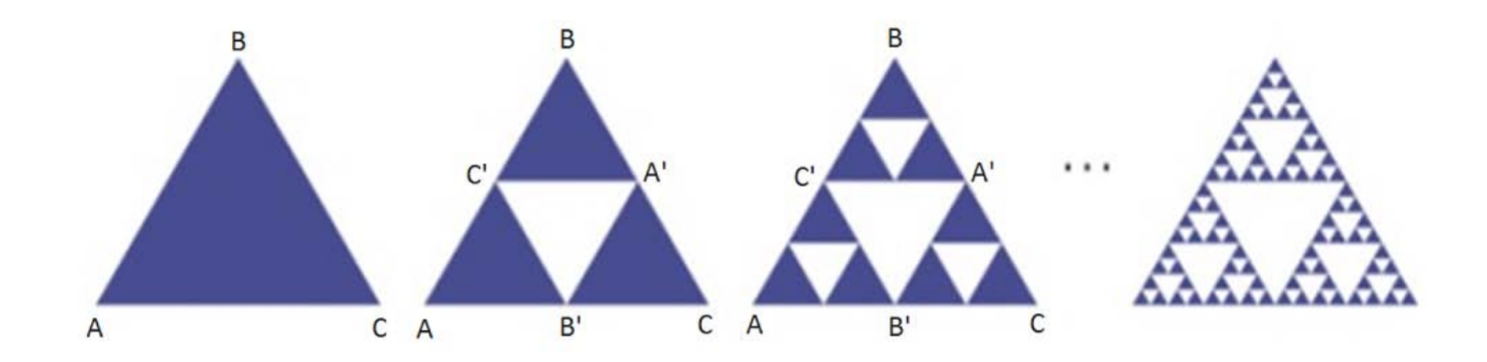
\includegraphics[scale=0.75]{chapter4/ima1.png}
\caption{Pasos del proceso de construcción del triangulo de $Sierpinsky$}
\label{fig:ima1}
\end{figure}
Hay muchas otras estructuras matemáticas definidas como fractal, como las curvas de   $Koch$,  el conjunto de $Cantor$ y el conjunto de $Mandelbrot$ que son presentados en la figura \ref{fig:ima2}. Son también ejemplos de fractales en la naturaleza, por ejemplo: nubes, montañas, hortalizas, árboles, La costa de continentes, islas entre otros.
\begin{figure}[h]
\centering
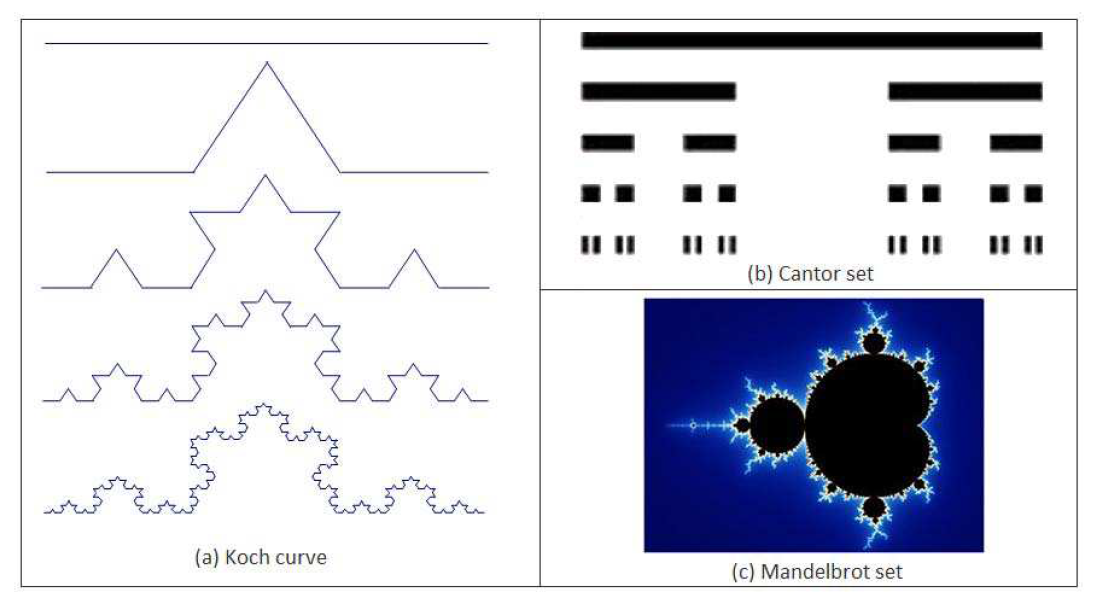
\includegraphics[scale=1.2]{chapter4/ima2.png}
\caption{Algunos ejemplos de fractales (a y b) fractales geométricos y (c) fractales algebraicos}
\label{fig:ima2}
\end{figure}


Los conceptos de fractal se han aplicado a varias tareas en el análisis de datos y la minería de datos. Una de ellas es la estimación de la dimensión intrínseca (D) de un conjunto de datos, que es relacionado  con el concepto de dimensión embebida (E) \cite{conf/pods/FaloutsosK94}.
\\\\
\textbf{Definición 3.1 Dimensión embebida  E:} Dado un conjunto finito de datos $A$, la  
dimensión embebida $E \in N$ es el número de atributos que definen $A$. Es decir, $E$ es la dimensión de el espacio en el que se encaja el conjunto de datos.
\\\\
\textbf{Definición 3.2 Dimensión intrínseca D:} Dado un conjunto de datos finitos $A$, su dimensión intrínseca
$D \in R^+$, es la dimensionalidad del objeto representado por los datos, independientemente de la
dimensión del espacio en el que está embebido.
\\\\
La dimensión intrínseca (D) es una medida de la cantidad de información que el conjunto de datos representa. Por ejemplo, la dimensión intrínseca de un conjunto de puntos distribuidos a lo largo de una linea  es igual a uno; si el conjunto está embebido  en un espacio dimensional superior, la dimensionalidad intrínseca   continúa igual a uno tal como se ilustra en la Figura \ref{fig:ima3}.

\begin{figure}[h]
\centering
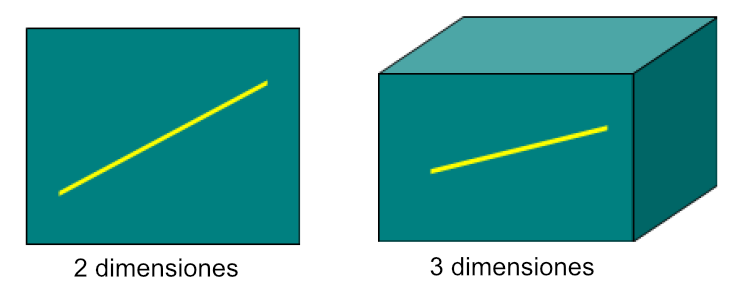
\includegraphics[scale=1.2]{chapter4/ima3.png}
\caption{Una linea embebida en dos o tres dimensiones donde $D=1$.}
\label{fig:ima3}
\end{figure}


Faloutsos & Kamel (1994) \cite{conf/pods/FaloutsosK94} propusieron el uso de la dimensión intrínseca como una herramienta para medir el comportamiento no uniforme de conjuntos de datos reales. Además, los autores presentaron estudios empíricos para demostrar que los datos reales suelen tener un comportamiento de auto-similitud, que es  una   característica fundamental de los objetos fractales. Por lo tanto, la dimensión intrínseca $D$ de un conjunto de datos real puede calcularse usando la dimensión fractal.

La dimensión intrínseca basada en la dimensión fractal ha sido empleada como una herramienta para el análisis de agrupamiento \cite{Barbara2003},  reglas de asociación temporal \cite{Barbara2004}, selección de atributos \cite{journals/jidm/TrainaTF10}, series cronológicas \cite{Chakrabarti:2002:FLA:584792.584797} y la minería de datos espaciales \cite{Traina:2001:TST:502512.502538}.

En este capítulo presentamos los principales conceptos relacionados con la teoría fractal que son usados en algunos de los métodos propuestos en esta tesis. La sección 2 muestra diferentes maneras de Calcular la dimensión fractal. El cálculo de correlación indicado por la correlación por la dimensión fractal se detalla en la Sección 3. La teoría fractal empleada para analizar   datos en la sección 3.

\section{Dimensión fractal}

Los fractales suelen tener características inusuales que pueden considerarse paradojas. Por ejemplo, el triángulo de $Sierpinski$ tiene un perímetro infinito (proporcional a $lim_{i\rightarrow\infty} (1+1/2)^i  $ ) y nulo (proporcional a $lim_{i\rightarrow\infty} (3/4)^i $) ya que a cada iteración de su proceso de construcción, que  teóricamente  es infinito, su perímetro aumenta y su área disminuye. Debido a estas propiedades, este fractal no puede ser considerado un objeto euclidiano unidimensional  (ya que su perímetro no es finito) ni un objeto euclidiano bidimensional (puesto que su área es nula). Así, es posible considerar una dimensionalidad de fraccionamiento llamada fractal \cite{di2016fractal}. Intuitivamente, la dimensión fractal del triángulo de $Sierpinski$ esta entre un valor de 1 y 2. Matemáticamente, el valor preciso es 1,58.

Hay varias definiciones para la dimensión fractal, que se presentan brevemente en este sección. La medida básica de la dimensión fractal se dedica a los fractales denominados exactamente auto-similares. Este tipo de fractal se compone de $M$ réplicas que son   una  versión reducida $1:s$ del fractal original.

\textbf{Definición 3.3 Dimensión fractal D:} Sea $M$ el número de réplicas y $s$ el factor de  escala
 por el que se reduce cada réplica, la dimensión fractal D de un fractal auto-similar es   definido en un espacio E-dimensional como:

\begin{equation}
D \equiv \frac{log M}{log s}
\label{eq:ec1}
\end{equation}

El triángulo de $Sierpinski$, por ejemplo, es un fractal exactamente auto-similar, porque su regla de construcción genera tres réplicas en escala $1:2$ en cada iteración. Por lo tanto, la dimensión fractal de $Sierpinski$ es $D = \frac{log 3}{log 2} \approx 1.58$. Similarmente, en la Figura \ref{fig:ima2}
el conjunto de Cantor conjunto y la curva de Koch son  fractales auto-similares con la dimensión fractal $ D = \frac{log2}{log3} \approx 0.63$ y $ D = \frac{log4}{log3} \approx 1.26$ respectivamente.

Esta definición de la dimensión fractal D es adecuada para Fractales  auto-similares matemáticamente  exactos. Sin embargo, para conjuntos de datos llamados  Fractales auto-similares estadísticamente, que no tienen reglas de construcción bien definidas, es más apropiado  calcular la dimensión fractal mediante el método de recuento de cajas (box-counting) \cite{Schroeder:1991}, que define la Correlación de Dimensión Fractal   $D_2$ tal como se presenta en Ecuación \ref{eq:ec2}

\textbf{Definición 3.4 Correlación de Dimensión Fractal $D_2$:} Dado un conjunto de datos auto-similar en el rango de escalas $[r1, r2]$, su dimensión fractal de correlación $D_2 \rightarrow \left[ \mathbb{R}^{+} \right]$ se mide como

\begin{equation}
D_2 \equiv  \frac{\partial log (\sum_i C_{r,1}^2)}{\partial (r)} \qquad \:r \epsilon [r1,r2 ]
\label{eq:ec2}
\end{equation}
donde $r$ es el lado de las celdas en una (hiper) cuadrícula  que divide el espacio del  conjunto de datos, y $C_r,i$, es el recuento de puntos en la i-ésima celda.

De forma práctica, el valor derivado que define la dimensión fractal $D_2$ puede se obtiene mediante la construcción de la gráfica de recuento de bloques, que representa los valores de $\sum_i C_{r,1}^2$  y $log (r)$ en un gráfico. Para los conjuntos fractales, la curva resultante es lineal en un intervalo $(r1, r2)$ y la dimensión fractal $D_2$ se estima por la pendiente de la línea que mejor se ajusta al intervalo analizado.

La figura \ref{fig:ima4} muestra un conjunto de $6561$ puntos en el triangulo de $Sierpinski$  y la gráfico en la escala log-log de la suma de la ocupación cuadrada $\sum_i C_{r,1}^2$ contra el tamaño de la celda  (radio) $r$.

\begin{figure}[h]
\centering
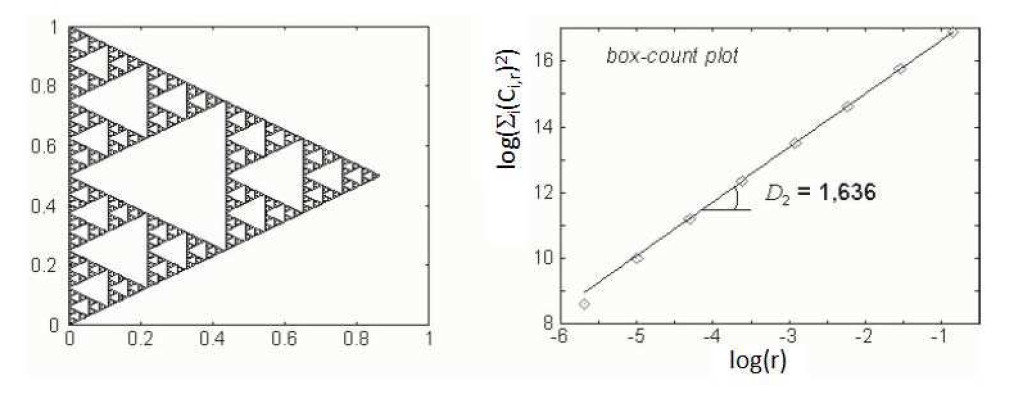
\includegraphics[scale=1.4]{chapter4/ima4.png}
\caption{El gráfico de conteo de cajas para el triangulo de $Sierpinki$.}
\label{fig:ima4}
\end{figure}

La dimensión fractal fue calculada por el algoritmo box-counting(), el cual tiene un coste lineal respecto al número de elementos en el conjunto de datos  \cite{DBLP:journals/jidm/TrainaTF10}. Este algoritmo es descrito en la siguiente sección. 

\section{Algoritmo de Calculo de la Dimensión Fractal}
 
Esta sección presenta un algoritmo para calcular la dimensión fractal D de cualquier conjunto dado de puntos en cualquier espacio E-dimensional. Una manera práctica de estimar D a partir de un conjunto de datos espaciales está utilizando el método de "recuento de cajas"  \cite{schroederpower}. Teóricamente, este método da una aproximación cercana a la dimensión fractal  \cite{DBLP:journals/jidm/TrainaTF10} \cite{traina1999distance}. Uno de los mejores algoritmos publicados para calcular D de un conjunto de datos es un algoritmo O (N log (N)), donde N es el número de puntos en el conjunto de datos \cite{belussi1998estimating}.  


Sin embargo, hemos desarrollado un nuevo, muy rápido, O (N) algoritmo para su implementación, que se presenta a continuación. Considere el espacio de direcciones de un conjunto de puntos en un espacio E-dimensional e imponga una E-rejilla con cuadrículas de tamaño de lado r. Centrándose en la i-ésima célula, sea $C r, i$ el recuento ('ocupaciones') de los puntos 2 en cada celda. Luego, calcule el valor $S (r) = i C r, i$. La dimensión fractal es la derivada de log $(S (r))$ con respecto al logaritmo del radio. \\

Al asumir conjuntos de datos auto-similares, esperamos que esta derivada resulte en un valor constante. Así, podemos obtener la dimensión fractal D de un conjunto de datos que traza $S (r)$ en escalas log-log para diferentes valores del radio r, y calcular la pendiente de la línea resultante. Es necesario procesar $S (r)$ para una cantidad R de valores de r, por lo que podemos lograr una aproximación estadística adecuada de la recta. Para evitar la lectura del conjunto de datos de nuevo para cada valor del radio, proponemos crear una estructura de cuadrícula de niveles múltiples, donde cada nivel tiene un radio de la mitad del tamaño del nivel anterior $(r = 1, 1/2, 1 / 4, 1/8, etc.)$. Cada nivel de la estructura corresponde a un radio diferente, por lo que la profundidad de la estructura es igual al número de puntos en el gráfico resultante. \\

La estructura se crea en la memoria principal, por lo que el número de puntos en el gráfico está limitado por la cantidad de memoria principal disponible. Si este gráfico es lineal para un rango adecuado de radios, el conjunto de datos es un fractal y su dimensión fractal D es la pendiente de la línea de ajuste de este gráfico. El algoritmo propuesto es lineal en el número de puntos en el conjunto de datos. La complejidad computacional del algoritmo es $O (N * E * R)$, donde N es el número de objetos en el conjunto de datos, E es la dimensionalidad de inclusión y R es el número de puntos utilizados para representar la función $S (r)$. Esto muestra que el algoritmo es escalable a conjuntos de datos de cualquier tamaño.\\

Para cada lado de celda dado r, sólo se mantienen las celdas que tienen al menos un punto ya procesado, contando la suma de ocupaciones $C r, i $ de esta celda. De esta manera, cada nuevo punto está directamente asociado a una célula en cada nivel, sin necesidad de ser comparado con los puntos de lectura anteriores. La figura 2 muestra la estructura utilizada en el algoritmo para conjuntos de datos bidimensionales y tridimensionales.\\

El lado de celda más grande del espacio de puntos genera $2 n$ células. En el siguiente nivel, cada célula se divide en otras 2 n células, y así sucesivamente. Dado que siempre se conoce la posición de cada célula en el espacio, cada célula está representada por: la suma de ocupaciones $C r, i$ en esta celda, y los punteros a las celdas en el siguiente nivel cubierto por esta celda (véase la Figura 2 ). Esta estructura es una especie de multi-dimensional "quad-árbol" (oct-tree para un espacio 3D, o E-dim-árbol). La Figura 3 muestra un ejemplo de esta estructura para un conjunto de datos con cinco puntos en tres niveles en un espacio bidimensional.\\


\begin{figure}[h]
\centering
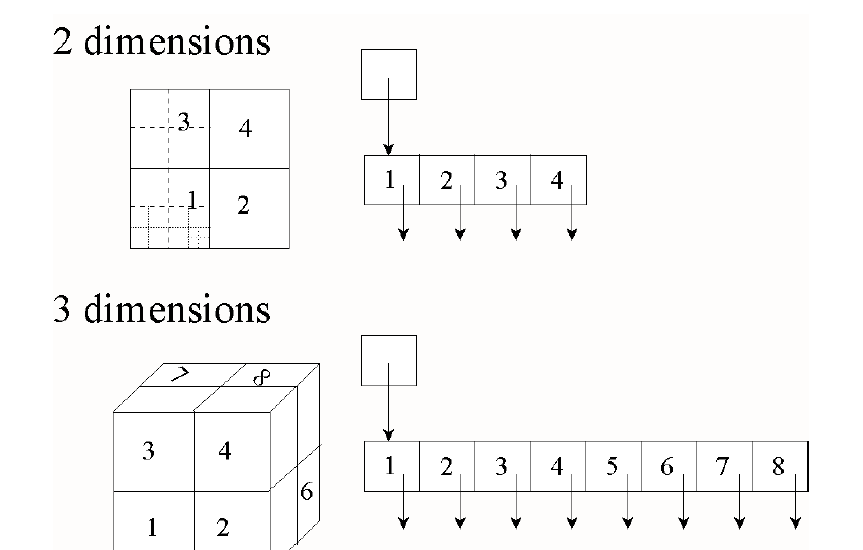
\includegraphics[scale=1.0]{chapter4/ima5.png}
\caption{ Representación de celdas de cuadrícula en espacios de 2 y 3 dimensiones. }
\label{fig:ima5}
\end{figure}
\\\\

Observe que se agregan nuevas celdas a la estructura cuando se solicita. Así, sólo se crean células ocupadas por al menos un punto $(C r, i> 0)$. El algoritmo procesa los puntos establecidos sólo una vez, por lo que es realmente muy rápido. El algoritmo 1 resume este proceso de cálculo.\\


\begin{figure}[h]
\centering
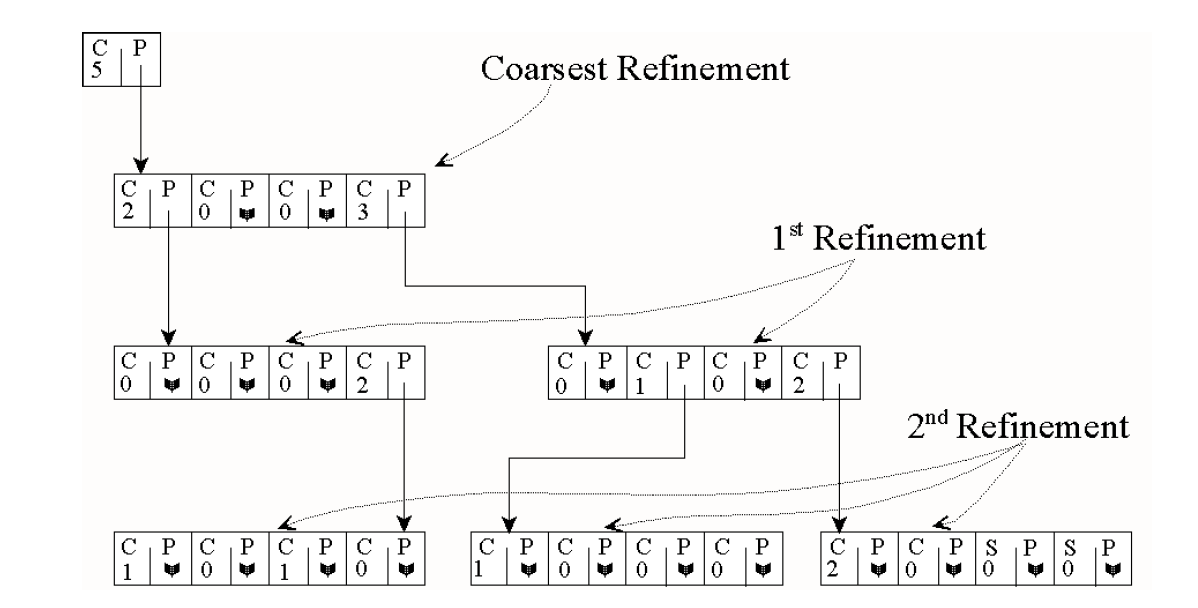
\includegraphics[scale=1.2]{chapter4/ima6.png}
\caption{Ejemplo de la estructura de datos utilizada para calcular la Suma de Ocupaciones de un conjunto de datos con 5 puntos (con tres niveles de resolución) }
\label{fig:ima6}
\end{figure}
 

\\\\
Observe que se agregan nuevas celdas a la estructura bajo demanda. Así, sólo las células ocupadas
Por al menos un punto $(C_{r,i}> 0)$. El algoritmo procesa sólo los puntos establecidos
Una vez, por lo que es realmente muy rápido. El algoritmo \ref{alg:algo1} resume este proceso de cálculo.
\\\\
\begin{algorithm}
\begin{algorithmic}[1]
\REQUIRE Normalizar el Dataset A(N filas, con E dimensiones/cada atributo)
\label{lin:lineaRara}
\ENSURE  Dimension fractal D
\FOR{Cada tamaño de grid deseaada $r = 1/2^j , j = 1,2, ...,l$}

    \FOR{Cada punto en el dataset}
    \STATE Decide cual celda del grid cae en (la i-esima celda)
    \STATE Incrementa la cuenta $C_i$
    \ENDFOR
    \STATE Procesa la sumatoria de los ocupados $S(r) = \sum C_i^2$
\ENDFOR

\STATE Imprime los valores de $log(r)$ y $log(S(r))$ generando un gráfico

\STATE Retorna la parte linear del gráfico cuesta abajo(regresión linear) de las dimensiones fractales D del dataset A

\end{algorithmic}
\caption{Procesar la dimensión fractal D del dataset A(conteo de cajas aproximadas)}
\label{alg:algo1}
\end{algorithm}
 
A medida que aumenta el lado de la cuadrícula, también aumenta el número de punteros a celdas vacías. Por lo tanto, para los conjuntos de datos de alta dimensión vale la pena mantener las celdas como listas enlazadas en lugar de arrays. Implementamos esta estructura como un objeto, usando una matriz para conjuntos de datos con la dimensión de incrustación menos o igual a tres, y usando una lista vinculada para conjuntos de datos con mayor dimensionalidad.	


\section{Consideraciones Finales}

